

\chapter{Sistema de controlo e monitorização}


Este capítulo tem como objetivo a descrição do sistema que resultou do trabalho prático
desta dissertação. Para esse fim, cada elemento pertencente ao sistema é caracterizado de
acordo com as suas funções e especificidades. É também descrito como os elementos interagem
entre si.




%Dashboard - Interface que apresenta a informação mais importante para o utilizador de forma apelativa, tornando mais fácil a interacção e respetiva leitura


% Mockups - Design que a plataforma deverá apresentar no fim do seu desenvolvimento.


\section{Descrição global do sistema}

Este sistema tem como objetivo a supervisão remota da produção de salicornia,  permitindo não só a monitorização dos dados adquiridos pelos sensores, como também da atuação remota de determinados comandos. Neste contexto também será possível a aquisição de imagens que possibilitará a deteção de intrusos nas quintas onde se produz esta espécie.

O esquema da figura \ref{componentesall} ilustra todos os componentes de um modo geral e as diferentes plataformas com que o cliente pode interagir. 

\begin{figure}[!htb]
	\centering
	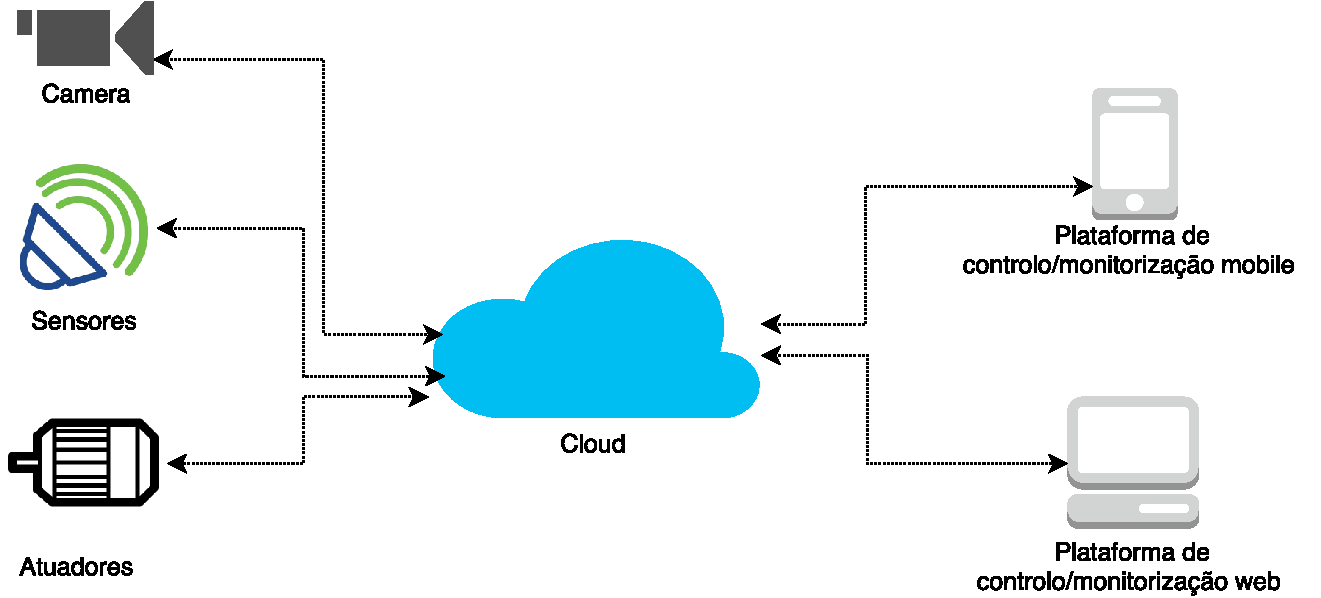
\includegraphics[scale=0.45]{esquemas/global_arquitetura.pdf}
	\caption{Ilustração principais componentes}
	\label{componentesall}
\end{figure}

Como vimos no capitulo 3, uma plantação de  salicórnia carece de um controlo relativamente fino de certos parâmetros ambientais sobretudo da salinidade do terreno onde ela cresce. A salinidade do terreno depende, por sua vez, das chuvas, da salinidade da água dos canais da ria. Nas quintas onde se cultiva salicórnia, a produção faz-se numa espécie de leiras limitadas por pequenos canais de irrigação. Esses canais podem ser cheios de água salgada proveniente dos esteiros que rodeiam a quinta. Essa operação implica a abertura de válvulas de admissão dessa água, medida do nível da maré nos canais, monitorização da qualidade e salinidade da água exterior.



\begin{figure}[!htb]
	\centering
	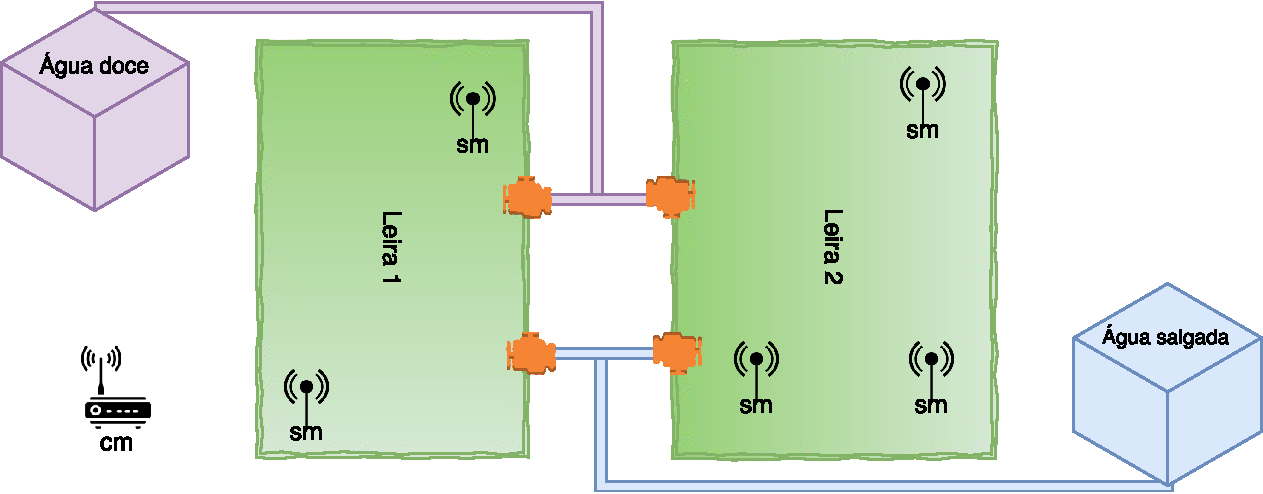
\includegraphics[scale=0.55]{esquemas/leiras-comm-geral.pdf}
	\caption{Ilustração de uma "quinta" onde se produz salicornia}
	\label{leira}
\end{figure}

A figura \ref{leira} ilustra esquematicamente a localização de duas leiras com determinados canais de irrigação para água doce e água salgada. 
 
 
Neste contexto, cada grupo de sensores espalhado por cada leira irá comunicar com um módulo central, originando uma topologia de rede em estrela.  Por sua vez, este módulo irá comunicar diretamente com a servidor que possibilitará que os dados sejam tratados e disponíveis para visualização ao cliente. Pressupõe-se portanto que este ultimo módulo tenha necessariamente ligação à rede de modo a conseguir consumir a API REST por HTTP desenvolvida para o efeito. 


\section{Componentes}

No contexto desta dissertação é necessário reter dois conceitos principais, são eles: 

\begin{itemize}
	\item \textbf{\textit{\ac{SM}}:} consiste num microcontrolador responsável pela aquisição de dados provenientes dos mais diversos tipos de sensores. Cada \textit{sensor module} terá que utilizar um determinado módulo de comunicação de modo a possibilitar a comunicação com um módulo central. Para além disso, pretende-se que o sensor module possa ter controlo sobre si, ou seja, inteligência própria.
	 
	\item \textbf{\textit{\ac{CM}}:} consiste num microcontrolador responsável pela receção dos dados preveniente dos \textit{sensor modules}. Pretende-se que este módulo envie informações para os sensor modules quando requisitados pelo utilizador. O principal objetivo deste módulo consiste em receber a informação proveniente dos sensor modules e respectivo envio para o servidor em cloud. 
	
	
\end{itemize}


A figura \ref{esquema1}, ilustra a comunicação entre três sensor modules com um controller moduler. Cada um desses sensor modules possui um conjunto especifico de sensores que comunica com controller module através de um determinado modulo de comunicação. Posteriormente, o controller module possui um determinado protocolo de comunicação que permite a utilização da API REST. 


\begin{figure}[h]
	\centering
	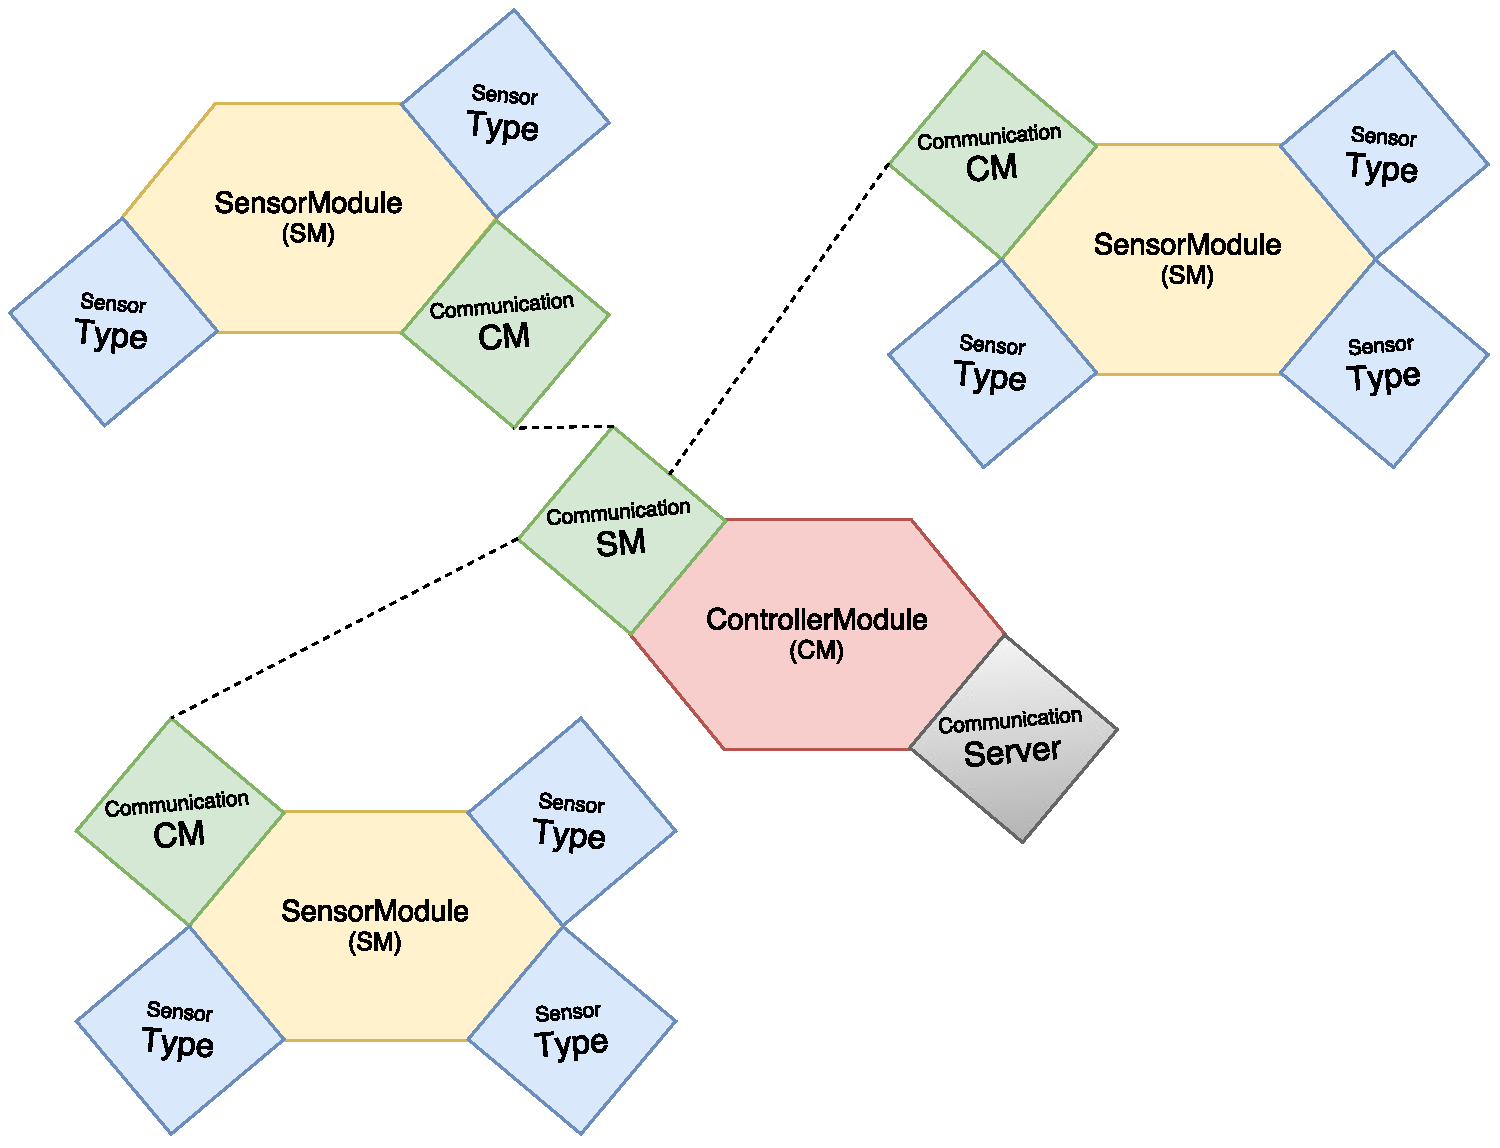
\includegraphics[scale=0.35]{esquemas/general-electronic-modules.pdf}
	\caption{Pirâmide do conhecimento: modelo DIKW}
	\label{esquema1}
\end{figure}


Seguidamente serão especificados todos os detalhes de cada modulo, uma vez que serão considerados na modulação deste sistema. 

\subsection{Controller Module}

nome
bateria
memoria
comunicacao
localizacao


\subsection{Sensor Module}


nome
tipos de senores 
tempo em que é recebida info 
bateria
localizacao



\newpage

\section{Design funcional}













\section{Considerações finais}